\documentclass{article}
\textheight 23.5cm \textwidth 15.8cm
%\leftskip -1cm
\topmargin -1.5cm \oddsidemargin 0.3cm \evensidemargin -0.3cm
%\documentclass[final]{siamltex}
\usepackage{ctex}
\usepackage{graphicx}
\usepackage{epsfig}
\usepackage{amsmath}
\usepackage{amsthm}
\usepackage{amssymb}
\usepackage{mathrsfs}
\usepackage{float}
\usepackage{multirow}
\usepackage{verbatim}
\usepackage{fancyhdr}
\usepackage{subfigure}
\usepackage{color}
\usepackage{mathtools}
\usepackage{mathrsfs}
%\usepackage{natbib}
\usepackage{sectsty}
%\usepackage[title]{appendix}
\usepackage{threeparttable}
\usepackage{dcolumn}
\usepackage{booktabs}
\usepackage{indentfirst}
\usepackage{setspace}
\usepackage{bm}
\usepackage{enumerate}
\usepackage{geometry}

\title{计算方法第二次程序作业报告}
\author{PB19071405\ 王昊元}
\date{2022 年 05 月 08 日}

\begin{document}
\maketitle

\section{问题描述}

分别使用向前Euler方法、向后Euler方法,和中心差方法,求解初值问题
\[
    \left\{
    \begin{aligned}
        & y'(x) = -100y, x \in [0, 0.2],\\
        & y(0) = 1.
    \end{aligned}
    \right.
\]
分别使用步长$h = \frac{1}{10}, \frac{1}{20}, \frac{1}{40}, \frac{1}{80}$,计算到$x = 0.2$.

\begin{enumerate}
    \item 画出数值解和准确解随$x\in [0, 0.2]$的变化规律,并利用数值结果进行稳定性描述。
    要求:分别对每一个数值方法,在一张图上画出准确解和不同网格的数值解,准确解使用曲线,
    数值解可以给出离散点的点图或者连接点的折线图。
    \item 对向后Euler方法,给出$x = 0.2$的误差表,并分析其精度。
\end{enumerate}

\section{数值计算方法}

\subsection{向前Euler方法}

用向前差商近似$y'(x)$,作$y(x)$的在$x = x_n$处的一阶向前差商,有
\[f(x_n, y(x_n)) = y'(x_n) \approx \frac{y(x_{n+1}) - y(x_n)}{h} \]
于是
\[y(x_{n+1}) = y(x_n) + hf(x_n, y(x_n))\]
得到计算$y(x_{n+1})$近似值$y_{n+1}$的\emph{向前Euler公式}:
\[y_{n+1} = y_n + hf(x_n, y_n)\]

\subsection{向后Euler方法}

作出$y(x)$的在$x = x_{n+1}$处的一阶向后差商,有
\[f(x_{n+1}, y(x_{n+1})) = y'(x_{n+1}) \approx \frac{y(x_{n+1}) - y(x_n)}{h} \]
于是
\[y(x_{n+1}) = y(x_n) + hf(x_{n+1}, y(x_{n+1}))\]
得到计算$y(x_{n+1})$近似值$y_{n+1}$的\emph{向后Euler公式}:
\[y_{n+1} = y_n + hf(x_{n+1}, y_{n+1})\]

\subsection{中心差方法}

作出$y(x)$的在$x=x_n$处的中心差商
\[f(x_n, y(x_n)) = y'(x_n) \approx \frac{y(x_{n+1}) - y(x_{n-1})}{2h}\]
于是得到计算$y(x_{n+1})$近似值$y_{n+1}$的\emph{中心差商格式}:
\[y_{n+1} = y_{n-1} + 2hf(x_n, y_n)\]

从公式中我们可以看出,需要知道$y_{n-1}, y_n$的值才能计算$y_{n+1}$的值,
所以我们需要先通过其他公式算出$y_1$,然后才能使用中心差方法,即起步运算。
这里起步运算采用向前Euler公式计算。

\section{结果及分析} \label{result_analyse}

\begin{enumerate}
    \item 每种数值计算方法的数值解及稳定性分析如下:
    \begin{enumerate}
        \item 向前Euler方法
        \begin{figure}[H]
            \centering
            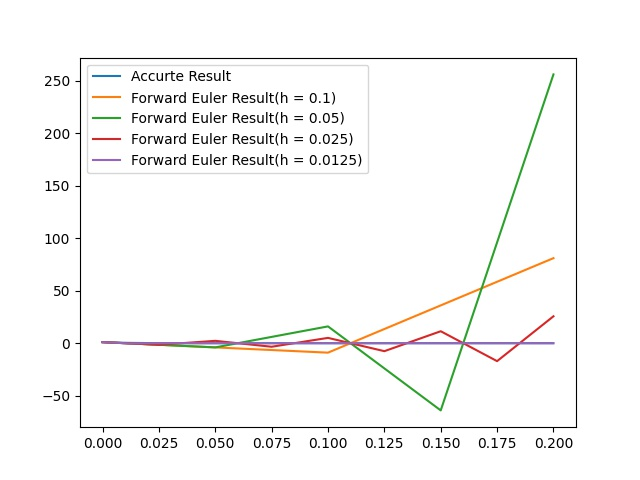
\includegraphics[width=0.7\textwidth]{../fig/forward_euler.jpg}
            \caption{向前Euler方法数值解及准确解}
            \label{forward_euler}
        \end{figure}
        从图\refeq{forward_euler}中可以看到,当$h = 0.1, 0.05, 0.025$时,
        数值计算结果在准确值上下波动,而且误差越来越大,表现出不稳定;而当$h = 0.0125$时
        数值结果几乎与准确结果重合(因作图时先作的蓝色准确解曲线,所以图中不太能看到蓝色曲线),
        为避免由于作图原因导致误判(如误差小但不稳定的情况),
        图\refeq{forward_euler_0.0125}为$h = 0.0125$的向前Euler方法数值计算结果。
        \begin{figure}[H]
            \centering
            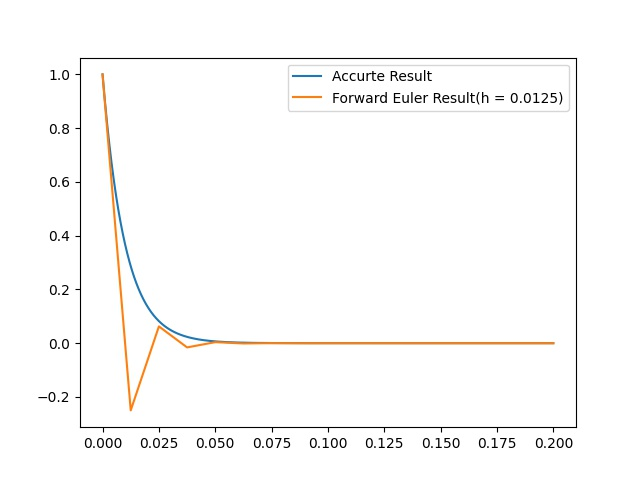
\includegraphics[width=0.7\textwidth]{../fig/forward_euler_h_0.0125.jpg}
            \caption{$h = 0.0125$的向前Euler方法}
            \label{forward_euler_0.0125}
        \end{figure}
        可以看到,当$h = 0.0125$时,向前Euler方法确实是稳定的。

        向前Euler方法的稳定性条件为$h \leq -\frac{2}{\lambda}$,
        对于该问题$\lambda = -100$,有在$h \leq 0.02$时向前Euler方法稳定,与从图中的分析结果相符。
        \item 向后Euler方法
        \begin{figure}[H]
            \centering
            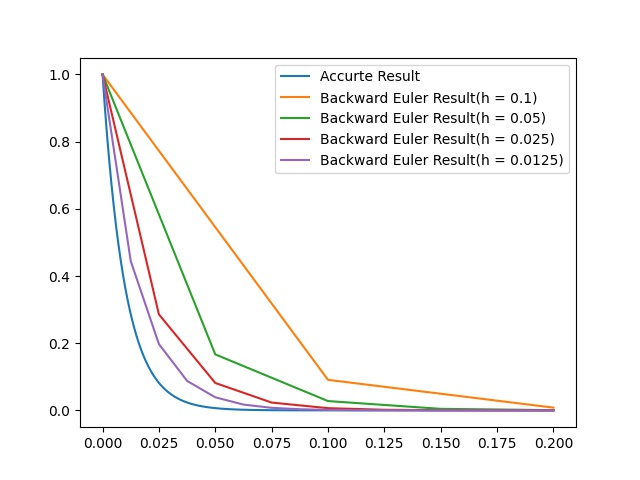
\includegraphics[width=0.7\textwidth]{../fig/backward_euler.jpg}
            \caption{向后Euler方法数值解及准确解}
            \label{backward_euler}
        \end{figure}
        从图\refeq{backward_euler}中可以看到,不论$h$取何值,数值计算结果的变化趋势
        与准确结果一致,且变化速度的变化趋势也一致,表现出在$h$取任何值时向后Euler方法都是稳定的。

        向后Euler方法的稳定性条件为$\lambda < 0$,在本题中满足,故对于任意步长向后Euler方法搜时稳定的。

        此外,可以看到,当步长越来越小时,数值计算误差越来越小。
        \item 中心差方法
        \begin{figure}[H]
            \centering
            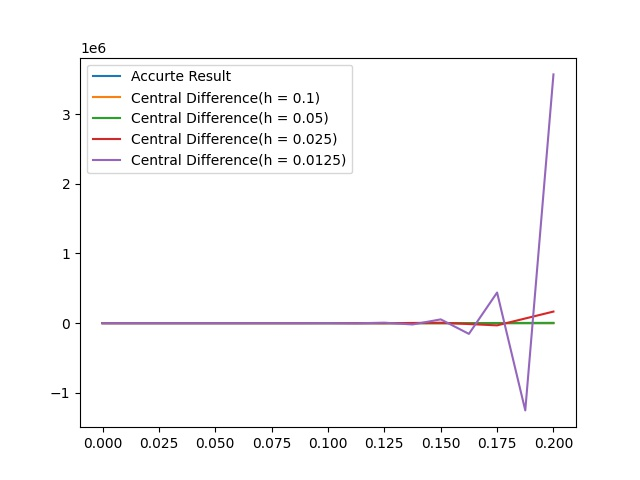
\includegraphics[width=0.7\textwidth]{../fig/central_difference.jpg}
            \caption{中心差方法数值解及准确解}
            \label{central_difference}
        \end{figure}
        从图\refeq{central_difference}中,可以看到,当$h = 0.05, 0.025, 0.0125$时,
        数值计算结果在准确值上下波动,而且误差越来越大,表现出不稳定;
        当$h = 0.1$时,数值计算结果的图像与准确解图像几乎重合,为消除作图纵轴值域太大
        导致误差在视觉上减小的影响,图\refeq{central_difference_0.1}为$h = 0.1$的中心差方法数值计算结果。
        \begin{figure}[H]
            \centering
            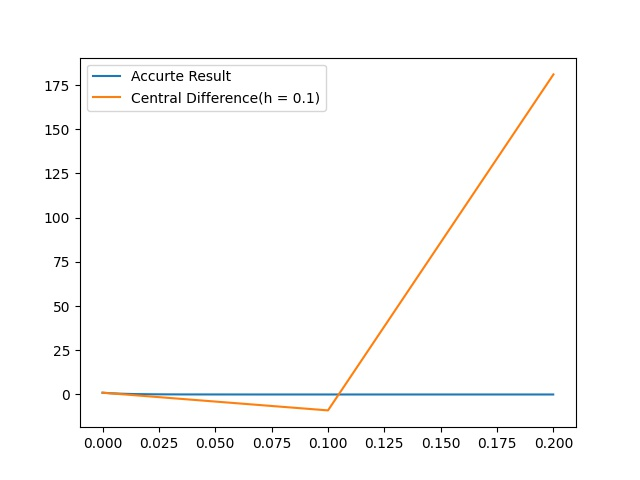
\includegraphics[width=0.7\textwidth]{../fig/central_difference_h_0.1.jpg}
            \caption{$h = 0.1$的中心差方法}
            \label{central_difference_0.1}
        \end{figure}
        从图\refeq{central_difference_0.1}可以看出,当$h = 0.1$时,中心差方法计算结果同样
        在准确解上下波动,误差同样在增大,表现为不稳定。

        中心差方法时无条件不稳定的,与以上的分析一致。
    \end{enumerate}

    \item 对于向后Euler方法在$x=0.2$的误差精度表如下:
    \begin{table}[H]
        \centering
        \caption{向后Euler方法在$x=0.2$的误差精度表}
        \begin{tabular}{ccccc}
            \hline
            h & 0.1 & 0.05 & 0.025 & 0.0125 \\
            \hline
            error & 8.26446075e-03 & 7.71602877e-04 & 4.44053694e-05 & 2.31575887e-06 \\
            \hline
            order & ~ & 3.42099026 & 4.11905248 & 4.26117719 \\
            \hline
        \end{tabular}
    \end{table}
\end{enumerate}

\section{结论}

主要且细节的分析在第\refeq{result_analyse}部分已经做过详细分析,这里就简单总结一下。
\begin{enumerate}
    \item 在实际计算中,我们希望某一步产生的扰动值在后面的计算中能够被控制,甚至逐步衰减,
    也就是我们希望所使用的数值计算方法是稳定的。
    对于本次程序作业所涉及的三种数值计算方法,
    \begin{itemize}
        \item 向前Euler方法是条件稳定的,稳定性条件是$h \leq -\frac{2}{\lambda}$
        \item 向后Euler方法在$\lambda < 0$的情况下是恒稳定(无条件稳定)的
        \item 中心差方法是无条件不稳定的
    \end{itemize}
    \item 对于稳定的数值计算方法,步长越小,截断误差越小;
    但同时使得计算量增加,导致舍入误差增大。
    不过由于目前大多数计算机有足够多的有效数字,在通常情况下舍入误差不会占主导地位。
\end{enumerate}


\end{document}
